% ============================================================================
% CHAPITRE 5 — SPRINT 3 : AGENT LLM ET PLANIFICATION CONVERSATIONNELLE
% ============================================================================

\section{Introduction}

Ce chapitre détaille le déroulement du Sprint~3 du projet Guidni. Ce troisième Sprint, d'une
durée de quatre semaines (décembre 2024), est consacré à l'implémentation de l'agent LLM
basé sur LangGraph et à la planification conversationnelle. Pour cela, j'ai suivi le plan
suivant~:
\begin{enumerate}
    \item Planning du Sprint
    \item Analyse
    \item Conception
    \item Réalisation
    \item Sprint Review
\end{enumerate}


% ────────────────────────────────────────────────────────────────
\section{Planning du Sprint~3}
% ────────────────────────────────────────────────────────────────

\subsection{Objectif du Sprint}

L'objectif du Sprint~3 est de construire le cerveau fonctionnel de Guidni~: l'Agent
Planificateur basé sur une machine à états LangGraph. Ce Sprint vise à substituer les
enchaînements procéduraux rudimentaires par un graphe d'états récursif capable d'adapter son
raisonnement dynamiquement. L'agent doit pouvoir orchestrer de manière autonome les outils de
recherche RAG, les appels météo, les calculs de distance et la génération de plans structurés.

\subsection{Sprint Backlog}

\begin{table}[H]
    \centering
    \caption{Sprint Backlog --- Sprint~3}
    \label{tab:sprint3_backlog}
    \small
    \begin{tabular}{c c p{7cm} c}
        \toprule
        \textbf{ID US} & \textbf{ID Task} & \textbf{Task} & \textbf{Complexité} \\
        \midrule
        US-01 & T-3.1 & Conception et implémentation de l'AgentState (TypedDict) & M \\[3pt]
        US-01 & T-3.2 & Implémentation du nœud THINK (raisonnement LLM) & XL \\[3pt]
        US-02 & T-3.3 & Implémentation du nœud EXECUTE\_TOOL (exécution des outils) & L \\[3pt]
        US-02 & T-3.4 & Implémentation du nœud VALIDATE (vérification du plan) & L \\[3pt]
        US-01 & T-3.5 & Implémentation du nœud RESPOND (formulation de la réponse) & M \\[3pt]
        US-02 & T-3.6 & Développement des 18 outils LLM-callable & XL \\[3pt]
        US-05 & T-3.7 & Intégration de l'outil \texttt{get\_weather} (Open-Meteo) & M \\[3pt]
        US-02 & T-3.8 & Intégration des outils RAG (rag\_search, rag\_search\_for\_plan) & L \\[3pt]
        US-01 & T-3.9 & Implémentation du système de mémoire conversationnelle & L \\[3pt]
        US-01 & T-3.10 & Implémentation de l'abstraction multi-fournisseurs LLM & M \\[3pt]
        US-03 & T-3.11 & Implémentation de la modification de plan par suivi conversationnel & M \\
        \bottomrule
    \end{tabular}
\end{table}

\subsection{Definition of Done (DoD)}

\begin{itemize}
    \item L'agent LangGraph démontre une conversation ininterrompue où il questionne la base,
    extrait des lieux et génère un plan structuré.
    \item Le graphe ne dépasse pas 15~itérations grâce aux garde-fous programmatiques.
    \item La mémoire conversationnelle gère les conversations longues par résumé automatique.
    \item L'abstraction multi-fournisseurs permet de basculer entre Ollama, Groq et Gemini.
\end{itemize}


% ────────────────────────────────────────────────────────────────
\section{Analyse}
% ────────────────────────────────────────────────────────────────

\subsection{Diagramme de cas d'utilisation}

\begin{figure}[H]
    \centering
    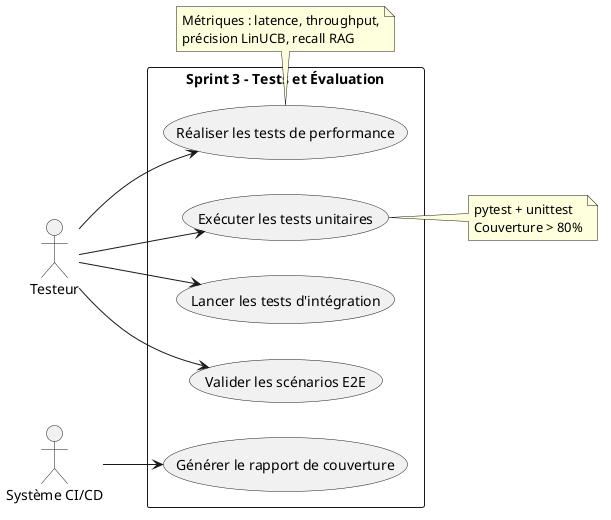
\includegraphics[width=0.85\textwidth]{diagrams/plantuml/usecase_sprint3.png}
    \caption{Diagramme de cas d'utilisation --- Sprint~3}
    \label{fig:uc_sprint3}
\end{figure}

\subsection{Description textuelle des cas d'utilisation}

\begin{table}[H]
    \centering
    \caption{Description textuelle --- CU : Générer un plan de voyage}
    \label{tab:cu_sprint3_1}
    \small
    \begin{tabular}{p{3cm} p{10cm}}
        \toprule
        \textbf{Champ} & \textbf{Description} \\
        \midrule
        Titre & Générer un plan de voyage multi-jours \\[3pt]
        Acteur & Touriste \\[3pt]
        Pré-condition & L'utilisateur est connecté, une conversation existe \\[3pt]
        Scénario nominal &
        1. Le touriste formule une demande de voyage (ex.\ : «\,3 jours à Djerba en famille\,») \newline
        2. Le nœud THINK raisonne et décide des outils à appeler \newline
        3. EXECUTE\_TOOL exécute les recherches (activités, hébergements, météo, distances) \newline
        4. Le cycle THINK → EXECUTE\_TOOL se répète jusqu'à satisfaction \newline
        5. \texttt{create\_plan\_structure()} construit le squelette du séjour \newline
        6. VALIDATE vérifie la cohérence (doublons, créneaux, budget) \newline
        7. RESPOND sauvegarde le plan dans \texttt{GeneratedPlan} et le retourne \\[3pt]
        Post-condition & Un plan validé est persisté en base et affiché au touriste \\
        \bottomrule
    \end{tabular}
\end{table}

\begin{table}[H]
    \centering
    \caption{Description textuelle --- CU : Modifier un plan existant}
    \label{tab:cu_sprint3_2}
    \small
    \begin{tabular}{p{3cm} p{10cm}}
        \toprule
        \textbf{Champ} & \textbf{Description} \\
        \midrule
        Titre & Modifier un plan existant par message de suivi \\[3pt]
        Acteur & Touriste \\[3pt]
        Pré-condition & Un plan actif existe pour la conversation courante \\[3pt]
        Scénario nominal &
        1. Le touriste envoie un message de modification (ex.\ : «\,Remplace le restaurant du jour 2\,») \newline
        2. L'agent charge le plan actif depuis la base \newline
        3. Le nœud THINK identifie les modifications nécessaires \newline
        4. \texttt{modify\_plan()} amende le plan itérativement \newline
        5. L'ancien plan est désactivé (\texttt{isActive=False}) \newline
        6. Le nouveau plan est sauvegardé avec \texttt{version} incrémenté \\[3pt]
        Post-condition & Le nouveau plan versionné est actif et affiché \\
        \bottomrule
    \end{tabular}
\end{table}


% ────────────────────────────────────────────────────────────────
\section{Conception}
% ────────────────────────────────────────────────────────────────

\subsection{Diagramme de séquence --- Cycle complet de l'agent}

Le diagramme suivant illustre le flux d'exécution complet d'un cycle de l'agent
planificateur, depuis la réception du message jusqu'à la génération du plan validé.

\begin{figure}[H]
    \centering
    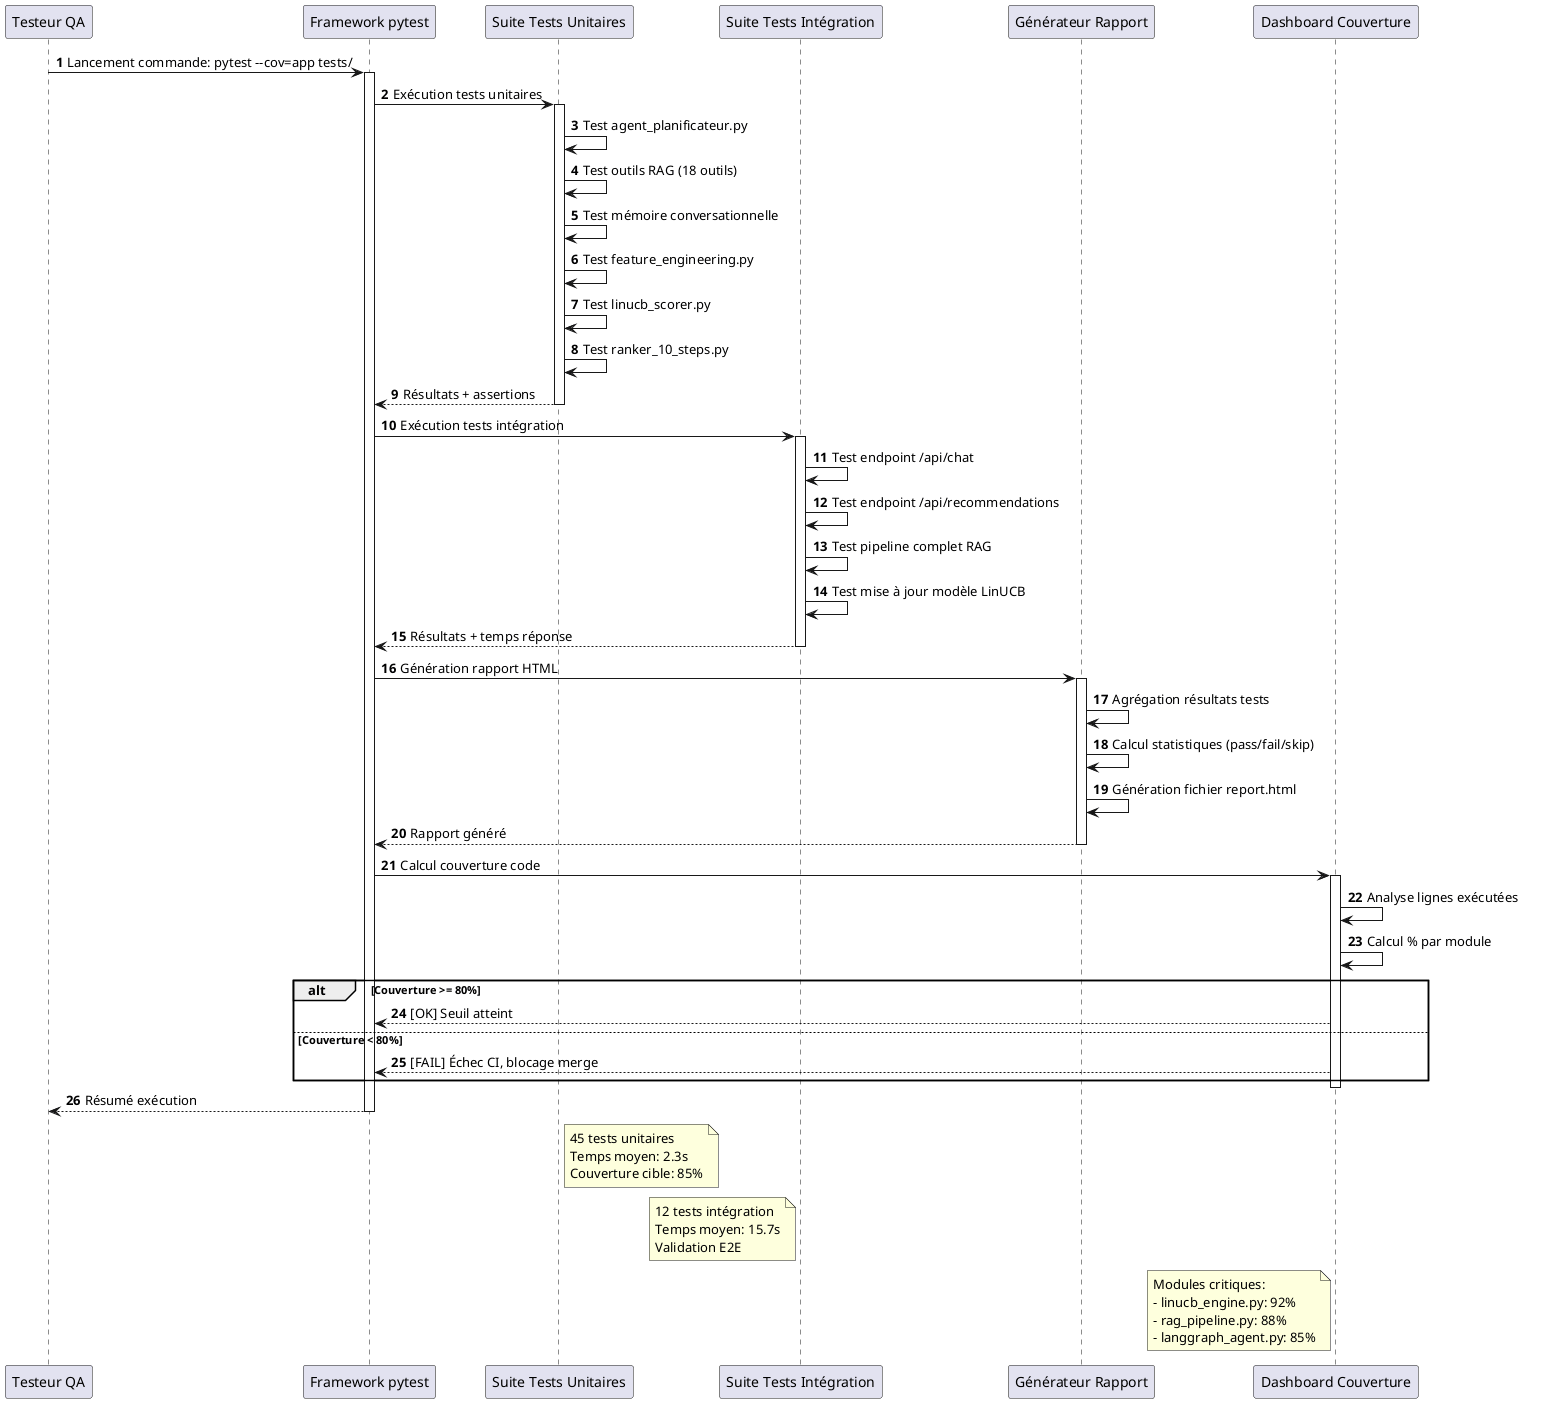
\includegraphics[width=\textwidth]{diagrams/plantuml/sequence_sprint3_primary.png}
    \caption{Diagramme de séquence --- Cycle complet de l'agent planificateur}
    \label{fig:seq_sprint3_primary}
\end{figure}

\subsection{Diagramme de séquence --- Modification de plan}

\begin{figure}[H]
    \centering
    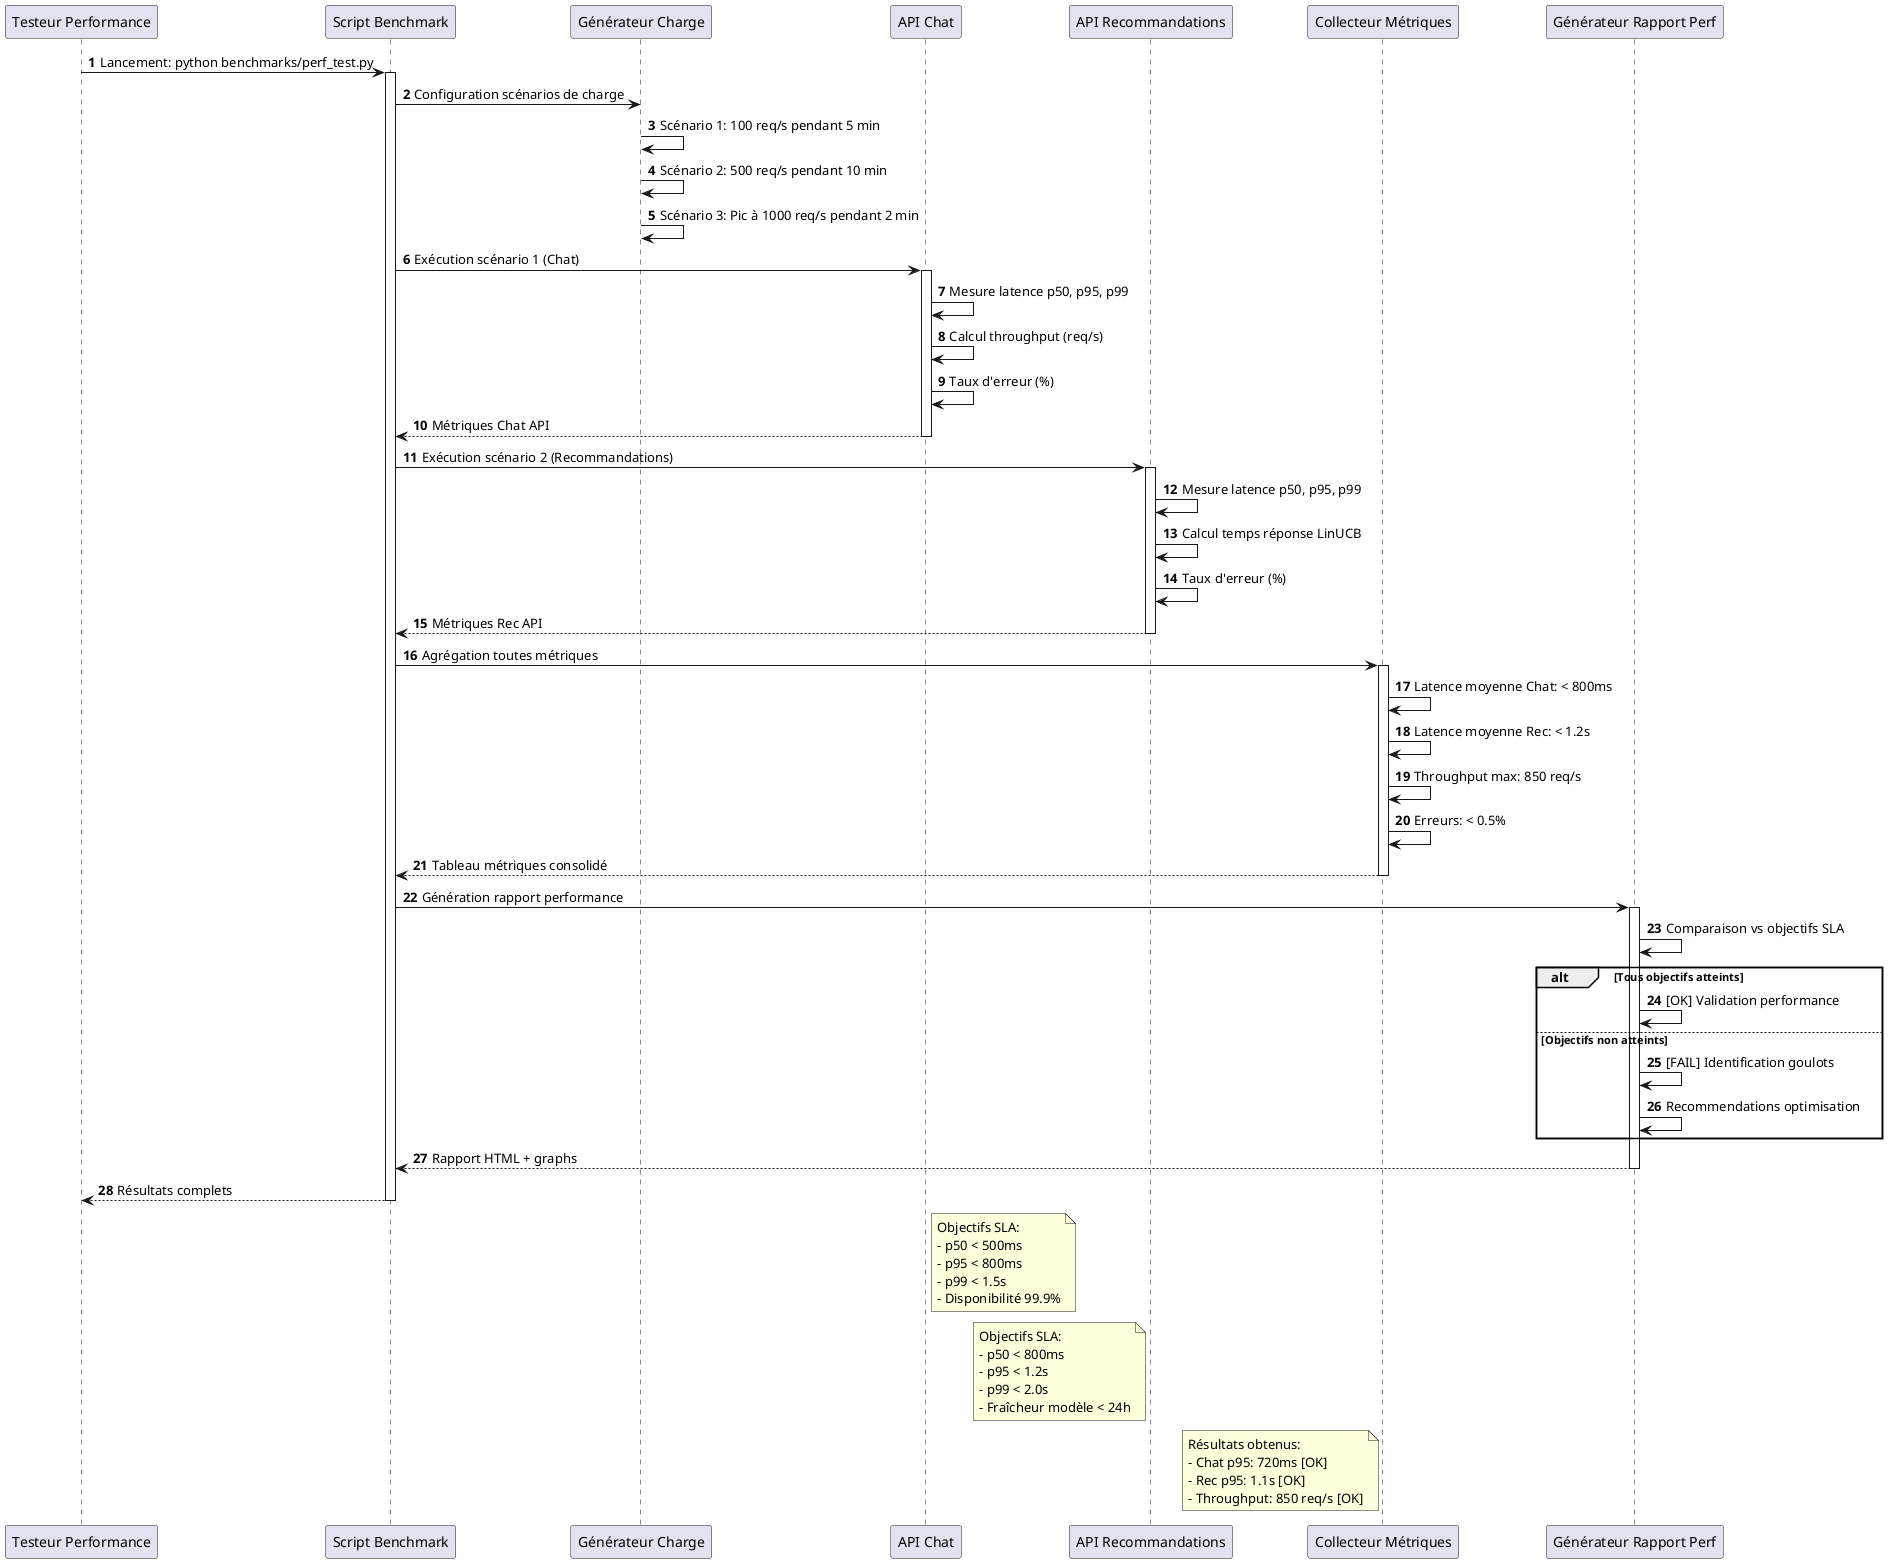
\includegraphics[width=\textwidth]{diagrams/plantuml/sequence_sprint3_secondary.png}
    \caption{Diagramme de séquence --- Modification d'un plan existant}
    \label{fig:seq_sprint3_secondary}
\end{figure}


% ────────────────────────────────────────────────────────────────
\section{Réalisation}
% ────────────────────────────────────────────────────────────────

\subsection{Machine à états LangGraph}

La machine à états de l'agent a été implémentée avec LangGraph. Le graphe articule quatre
nœuds principaux~: \textbf{THINK} interroge le LLM sélectionné, un routeur conditionnel
(\texttt{\_should\_continue()}) décide de la suite des opérations, \textbf{EXECUTE\_TOOL}
exécute l'outil appelé, \textbf{VALIDATE} vérifie la cohérence du plan, et \textbf{RESPOND}
formule la réponse finale. Après chaque exécution d'outil, le système reconduit l'agent vers
THINK pour réévaluation.

\begin{figure}[H]
    \centering
    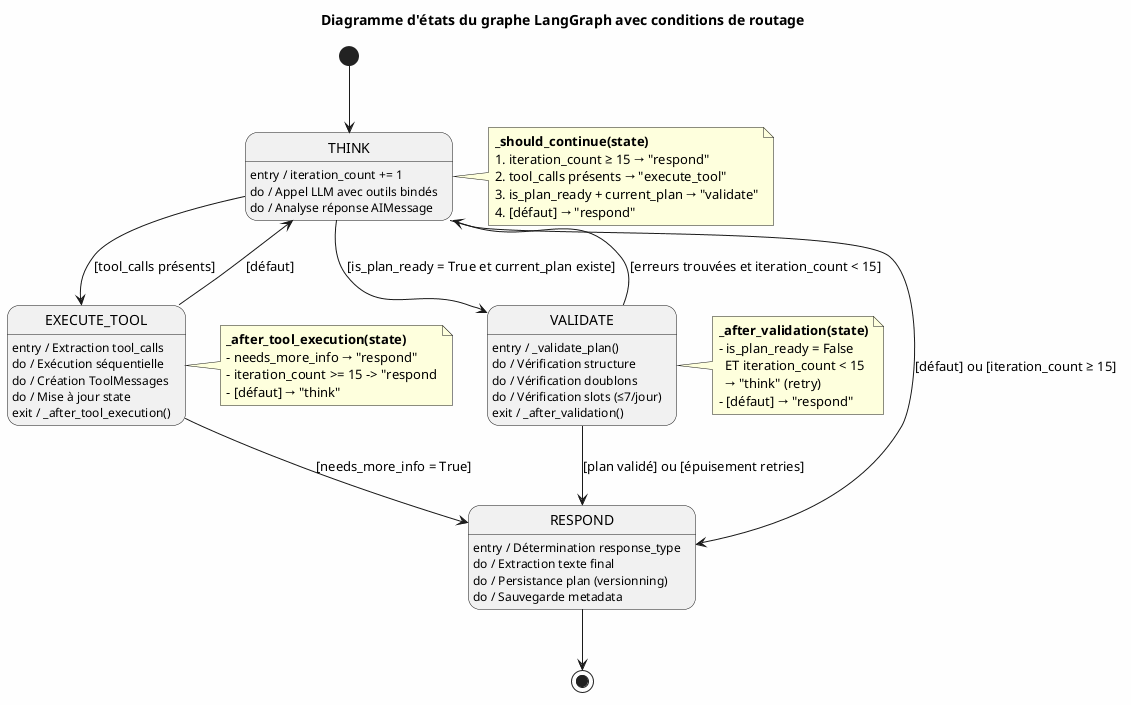
\includegraphics[width=0.75\textwidth]{diagrams/fig_04_langgraph_routing.png}
    \caption{Machine à états cyclique de l'agent planificateur}
    \label{fig:langgraph_graph}
\end{figure}

\subsection{Les 18 outils LLM-callable}

Un arsenal de dix-huit outils a été développé et enregistré dans un registre global~:

\begin{itemize}
    \item \textbf{Outils de recherche}~: \texttt{search\_activities}, \texttt{search\_stays},
    \texttt{search\_restaurants} pour la sélection géographique.
    \item \textbf{Outils contextuels}~: \texttt{get\_weather} (Open-Meteo),
    \texttt{get\_distance} (Haversine).
    \item \textbf{Outils RAG}~: \texttt{rag\_search}, \texttt{rag\_search\_for\_plan},
    \texttt{rag\_get\_similar} pour la recherche sémantique.
    \item \textbf{Outils de planification}~: \texttt{create\_plan\_structure},
    \texttt{modify\_plan}, \texttt{save\_plan\_tool} pour la construction du séjour.
    \item \textbf{Outil d'interaction}~: \texttt{ask\_user} pour questionner le touriste.
\end{itemize}

\subsection{Mémoire conversationnelle}

Le gestionnaire conversationnel emploie une politique de mémoire à taille glissante~: les
8~derniers messages sont systématiquement chargés. Lorsque la profondeur dépasse 15~messages,
un module résumeur contextuel extrait les points capitaux et se substitue aux messages anciens,
maintenant la cohérence sans surcharger le contexte du LLM.

\subsection{Abstraction multi-fournisseurs LLM}

Le patron fabrique (\textit{factory pattern}) implémenté dans \texttt{provider.py} permet
de basculer entre Ollama (local), Groq (rapide), Gemini (contexte long) et Lightning AI
via un simple paramètre de configuration, sans modification du code agentique.

\begin{table}[H]
    \centering
    \caption{Fournisseurs LLM intégrés dans Guidni}
    \label{tab:llm_providers}
    \small
    \begin{tabular}{p{2cm} p{3cm} p{1.5cm} p{2cm} p{4cm}}
        \toprule
        \textbf{Fournisseur} & \textbf{Modèle} & \textbf{Type} & \textbf{Latence} &
        \textbf{Caractéristique} \\
        \midrule
        Ollama & qwen2.5:7b & Local & 2--5\,s & Gratuit, hors-ligne \\[3pt]
        Groq & llama-3.3-70b & Cloud & 0.5--1\,s & Très rapide, 128k tokens \\[3pt]
        Gemini & gemini-2.5-flash & Cloud & 1--2\,s & Contexte 1M tokens \\[3pt]
        Lightning & openai/gpt-5 & Cloud & 1--3\,s & Dernière génération \\
        \bottomrule
    \end{tabular}
\end{table}

\subsection{Flux d'exécution des outils}

La figure suivante illustre le flux détaillé lorsqu'un outil est appelé par l'agent,
depuis la sélection par le LLM jusqu'au retour du résultat dans l'état.

\begin{figure}[H]
    \centering
    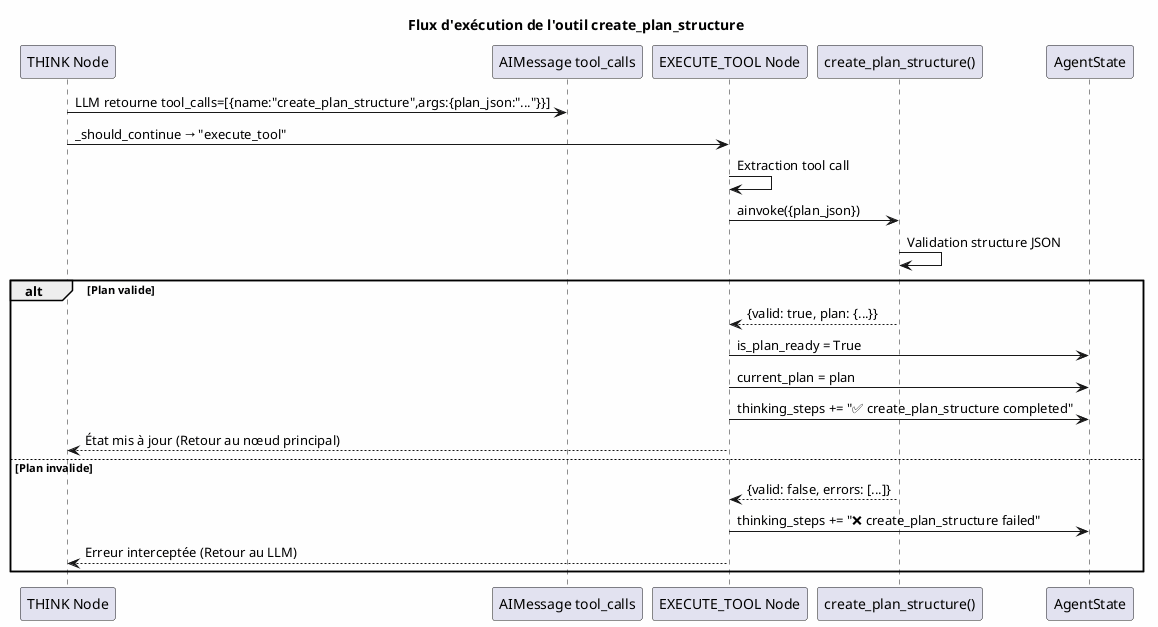
\includegraphics[width=0.85\textwidth]{diagrams/fig_04_tool_execution_flow.png}
    \caption{Flux d'exécution d'un outil par l'agent LangGraph}
    \label{fig:tool_exec_flow}
\end{figure}

\subsection{Démonstration de planification}

La figure suivante montre un exemple de conversation où l'agent génère un plan de 3~jours
à Djerba pour une famille, en orchestrant automatiquement les outils de recherche, météo
et planification.

\begin{figure}[H]
    \centering
    
\includegraphics[width=\textwidth]{diagrams/screen_04_chat_plan_output.png}
    \caption{Exemple de plan de voyage généré par l'agent}
    \label{fig:screen_plan}
\end{figure}

\begin{figure}[H]
    \centering
    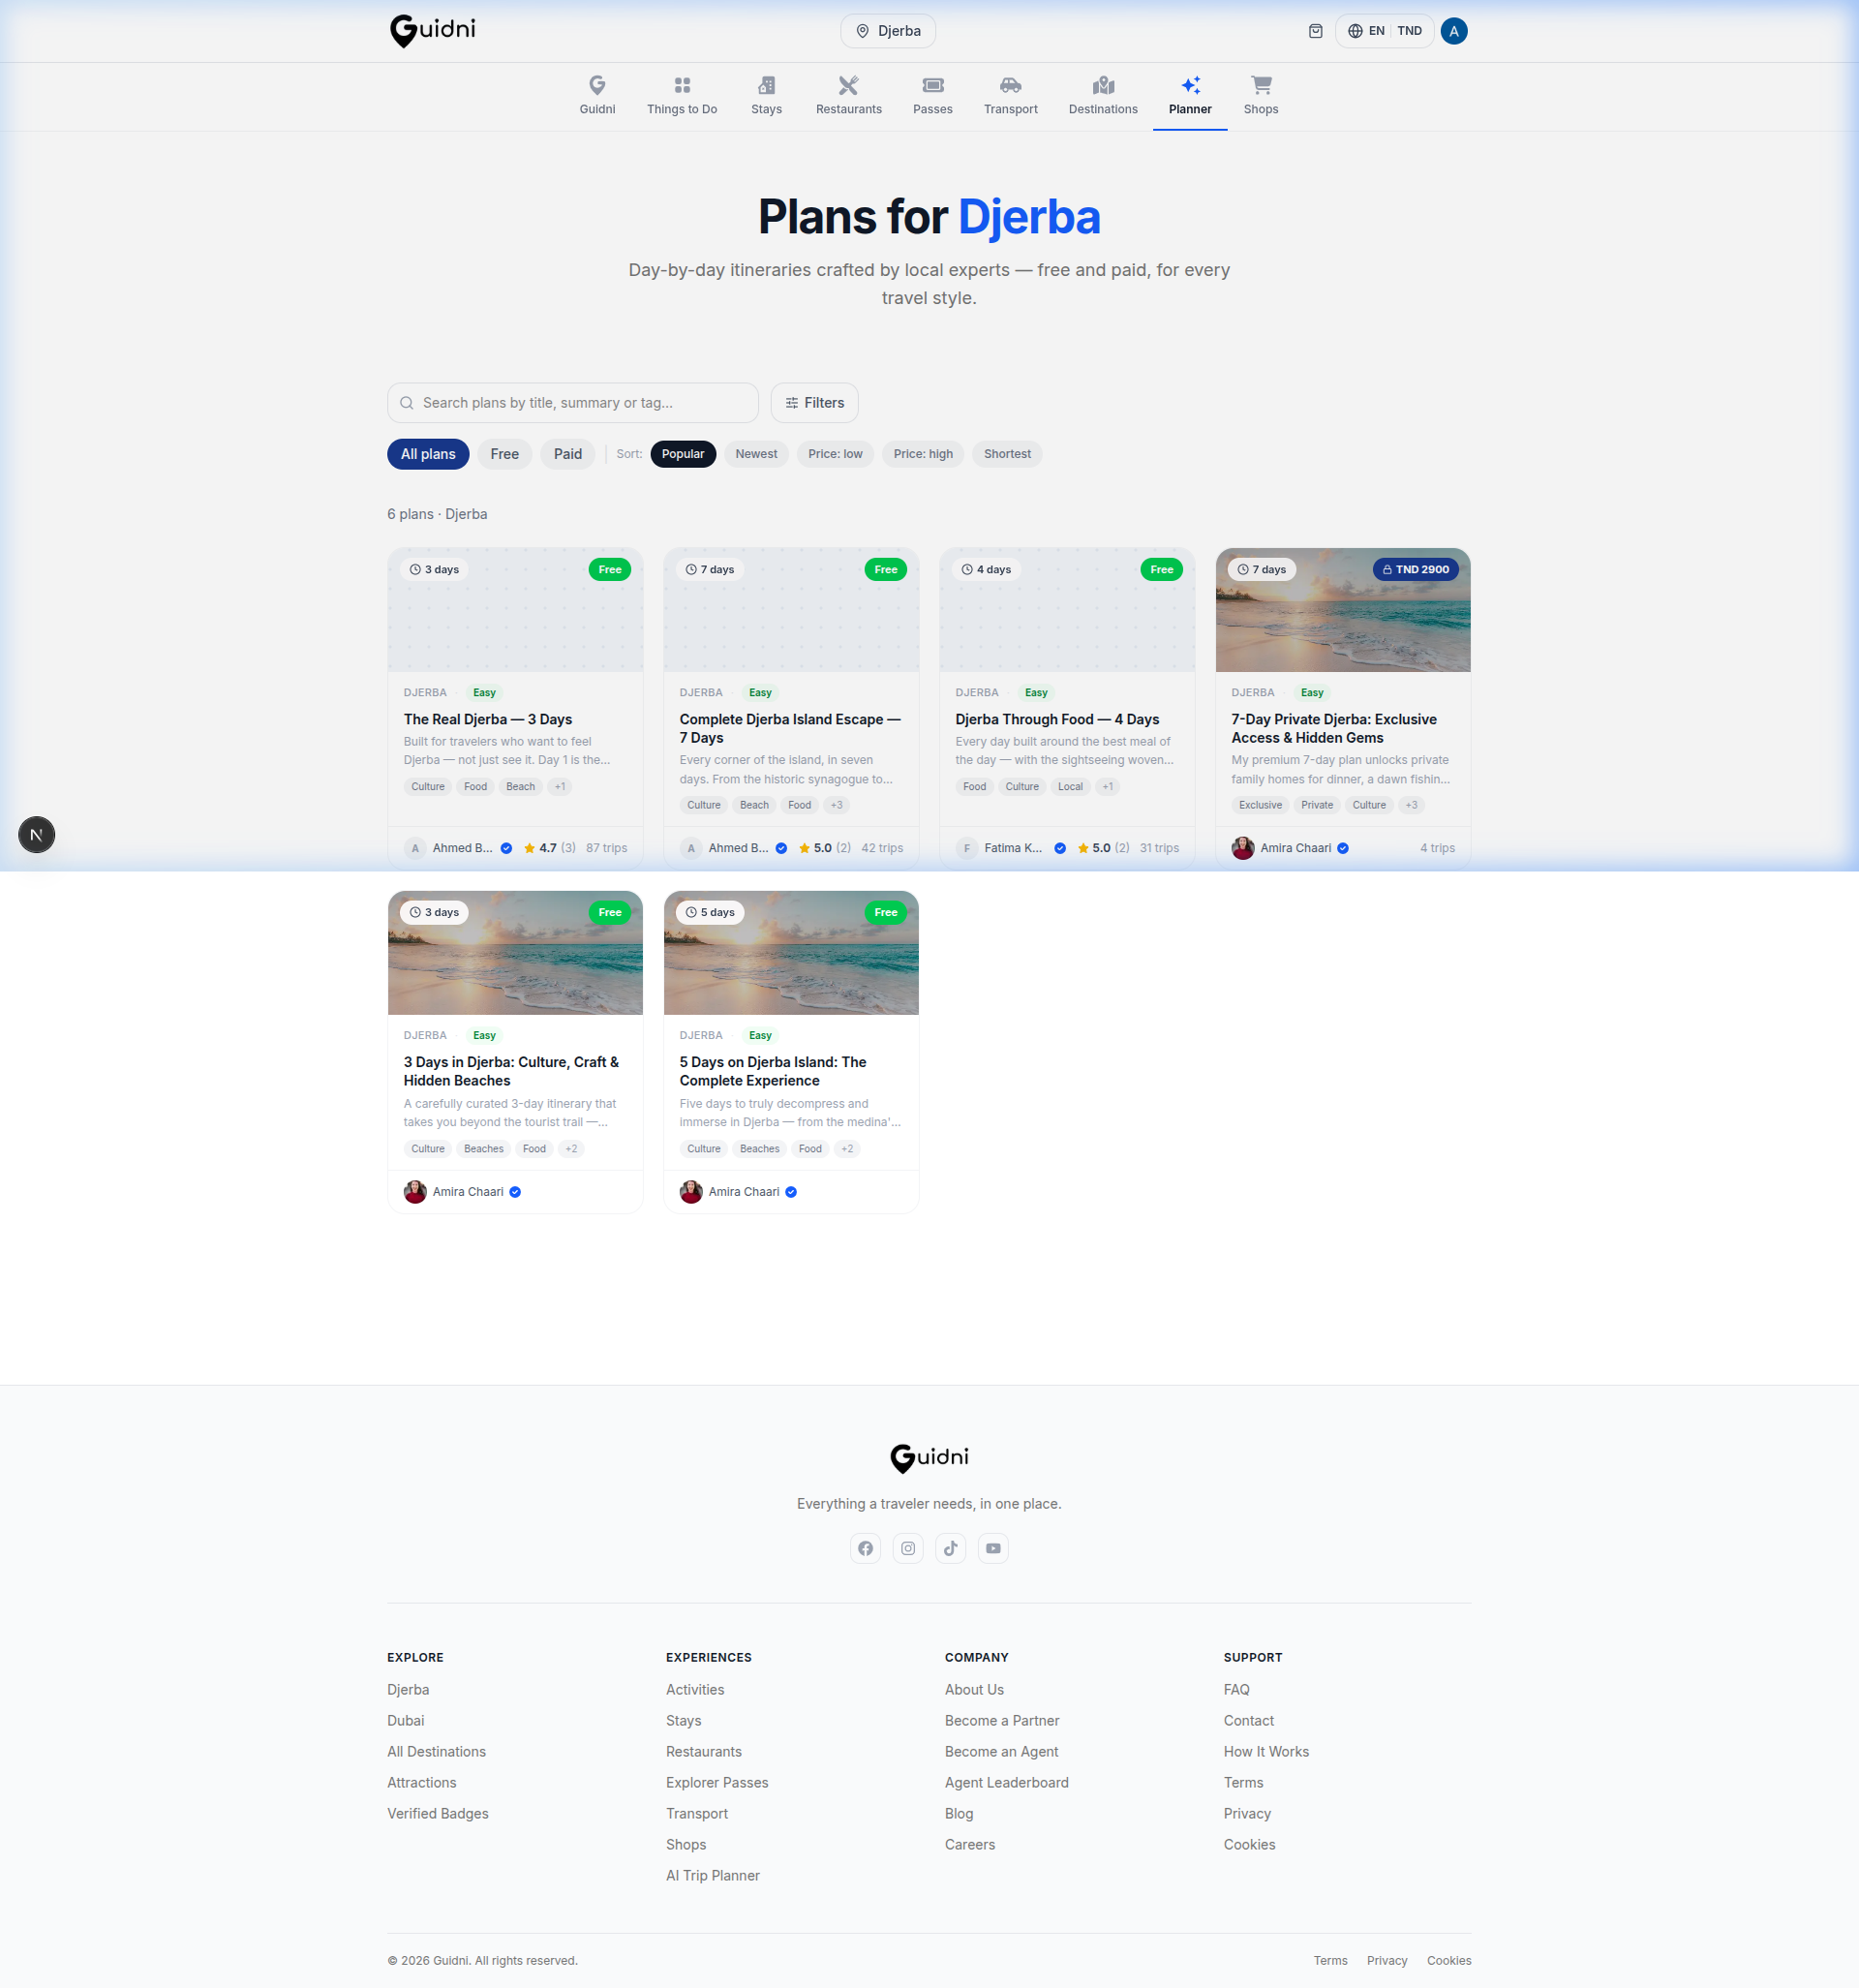
\includegraphics[width=\textwidth]{diagrams/screen_A4_plan_output_full.png}
    \caption{Plan de voyage complet affiché dans l'interface}
    \label{fig:screen_plan_full}
\end{figure}

\subsection{Étapes de raisonnement de l'agent}

La figure suivante montre les étapes de raisonnement (\textit{thinking steps}) visibles
dans les journaux du backend, attestant du cycle THINK $\rightarrow$ EXECUTE\_TOOL
$\rightarrow$ THINK successif avant la génération du plan final.

\begin{figure}[H]
    \centering
    
\includegraphics[width=\textwidth]{diagrams/screen_06_plan_thinking_steps.png}
    \caption{Étapes de raisonnement de l'agent planificateur}
    \label{fig:screen_thinking}
\end{figure}


% ────────────────────────────────────────────────────────────────
\section{Sprint Review}
% ────────────────────────────────────────────────────────────────

Lors de la Sprint Review, l'agent a fait la démonstration de sa robustesse en orchestrant une
dizaine d'appels d'outils successifs avant de produire un plan structuré validé. La
vérification des journaux détaillés a attesté le respect de la séquence cyclique du graphe et
des boucles de validation. L'encadrant a validé le Sprint.

Lors de la Sprint Retrospective, l'adoption de LangGraph a été jugée fructueuse pour la
transparence du raisonnement. L'équipe a identifié le besoin du moteur de recommandation
LinUCB pour gérer les interactions passives (navigation, défilement), justifiant le Sprint~4.


% ────────────────────────────────────────────────────────────────
\section*{Conclusion}
\addcontentsline{toc}{section}{Conclusion}

Le Sprint~3 a permis de construire le cœur intelligent de Guidni~: l'agent planificateur
LangGraph avec ses quatre nœuds, ses dix-huit outils et son système de mémoire
conversationnelle. L'abstraction multi-fournisseurs LLM offre une flexibilité de déploiement.
Le Sprint~4 sera consacré à l'implémentation du moteur de recommandation LinUCB, aux tests
d'évaluation et à la finalisation du système.
